\documentclass[1p]{elsarticle_modified}
%\bibliographystyle{elsarticle-num}

%\usepackage[colorlinks]{hyperref}
%\usepackage{abbrmath_seonhwa} %\Abb, \Ascr, \Acal ,\Abf, \Afrak
\usepackage{amsfonts}
\usepackage{amssymb}
\usepackage{amsmath}
\usepackage{amsthm}
\usepackage{scalefnt}
\usepackage{amsbsy}
\usepackage{kotex}
\usepackage{caption}
\usepackage{subfig}
\usepackage{color}
\usepackage{graphicx}
\usepackage{xcolor} %% white, black, red, green, blue, cyan, magenta, yellow
\usepackage{float}
\usepackage{setspace}
\usepackage{hyperref}

\usepackage{tikz}
\usetikzlibrary{arrows}

\usepackage{multirow}
\usepackage{array} % fixed length table
\usepackage{hhline}

%%%%%%%%%%%%%%%%%%%%%
\makeatletter
\renewcommand*\env@matrix[1][\arraystretch]{%
	\edef\arraystretch{#1}%
	\hskip -\arraycolsep
	\let\@ifnextchar\new@ifnextchar
	\array{*\c@MaxMatrixCols c}}
\makeatother %https://tex.stackexchange.com/questions/14071/how-can-i-increase-the-line-spacing-in-a-matrix
%%%%%%%%%%%%%%%

\usepackage[normalem]{ulem}

\newcommand{\msout}[1]{\ifmmode\text{\sout{\ensuremath{#1}}}\else\sout{#1}\fi}
%SOURCE: \msout is \stkout macro in https://tex.stackexchange.com/questions/20609/strikeout-in-math-mode

\newcommand{\cancel}[1]{
	\ifmmode
	{\color{red}\msout{#1}}
	\else
	{\color{red}\sout{#1}}
	\fi
}

\newcommand{\add}[1]{
	{\color{blue}\uwave{#1}}
}

\newcommand{\replace}[2]{
	\ifmmode
	{\color{red}\msout{#1}}{\color{blue}\uwave{#2}}
	\else
	{\color{red}\sout{#1}}{\color{blue}\uwave{#2}}
	\fi
}

\newcommand{\Sol}{\mathcal{S}} %segment
\newcommand{\D}{D} %diagram
\newcommand{\A}{\mathcal{A}} %arc


%%%%%%%%%%%%%%%%%%%%%%%%%%%%%5 test

\def\sl{\operatorname{\textup{SL}}(2,\Cbb)}
\def\psl{\operatorname{\textup{PSL}}(2,\Cbb)}
\def\quan{\mkern 1mu \triangleright \mkern 1mu}

\theoremstyle{definition}
\newtheorem{thm}{Theorem}[section]
\newtheorem{prop}[thm]{Proposition}
\newtheorem{lem}[thm]{Lemma}
\newtheorem{ques}[thm]{Question}
\newtheorem{cor}[thm]{Corollary}
\newtheorem{defn}[thm]{Definition}
\newtheorem{exam}[thm]{Example}
\newtheorem{rmk}[thm]{Remark}
\newtheorem{alg}[thm]{Algorithm}

\newcommand{\I}{\sqrt{-1}}
\begin{document}

%\begin{frontmatter}
%
%\title{Boundary parabolic representations of knots up to 8 crossings}
%
%%% Group authors per affiliation:
%\author{Yunhi Cho} 
%\address{Department of Mathematics, University of Seoul, Seoul, Korea}
%\ead{yhcho@uos.ac.kr}
%
%
%\author{Seonhwa Kim} %\fnref{s_kim}}
%\address{Center for Geometry and Physics, Institute for Basic Science, Pohang, 37673, Korea}
%\ead{ryeona17@ibs.re.kr}
%
%\author{Hyuk Kim}
%\address{Department of Mathematical Sciences, Seoul National University, Seoul 08826, Korea}
%\ead{hyukkim@snu.ac.kr}
%
%\author{Seokbeom Yoon}
%\address{Department of Mathematical Sciences, Seoul National University, Seoul, 08826,  Korea}
%\ead{sbyoon15@snu.ac.kr}
%
%\begin{abstract}
%We find all boundary parabolic representation of knots up to 8 crossings.
%
%\end{abstract}
%\begin{keyword}
%    \MSC[2010] 57M25 
%\end{keyword}
%
%\end{frontmatter}

%\linenumbers
%\tableofcontents
%
\newcommand\colored[1]{\textcolor{white}{\rule[-0.35ex]{0.8em}{1.4ex}}\kern-0.8em\color{red} #1}%
%\newcommand\colored[1]{\textcolor{white}{ #1}\kern-2.17ex	\textcolor{white}{ #1}\kern-1.81ex	\textcolor{white}{ #1}\kern-2.15ex\color{red}#1	}

{\Large $\underline{12n_{0288}~(K12n_{0288})}$}

\setlength{\tabcolsep}{10pt}
\renewcommand{\arraystretch}{1.6}
\vspace{1cm}\begin{tabular}{m{100pt}>{\centering\arraybackslash}m{274pt}}
\multirow{5}{120pt}{
	\centering
	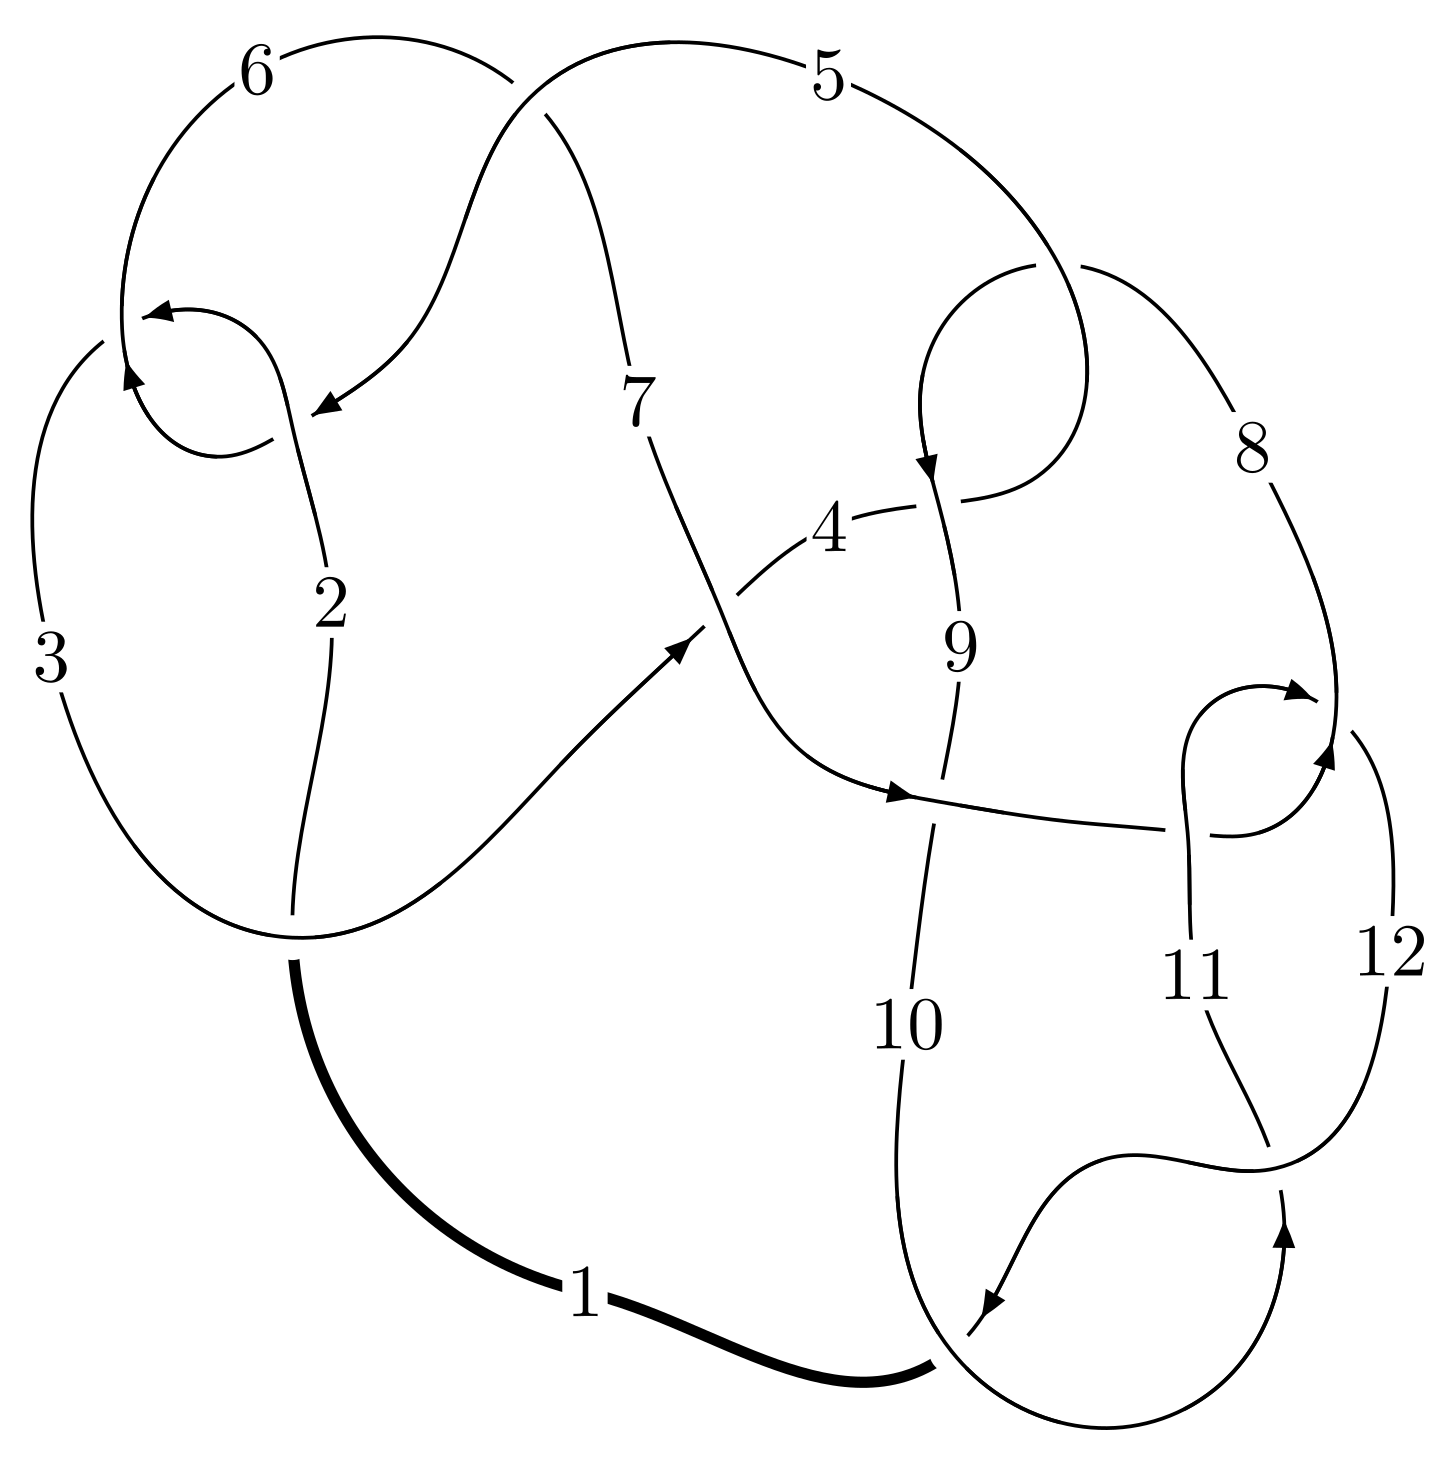
\includegraphics[width=112pt]{../../../GIT/diagram.site/Diagrams/png/2377_12n_0288.png}\\
\ \ \ A knot diagram\footnotemark}&
\allowdisplaybreaks
\textbf{Linearized knot diagam} \\
\cline{2-2}
 &
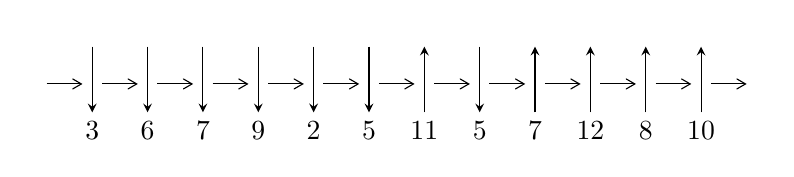
\begin{tikzpicture}[x=20pt, y=17pt]
	% nodes
	\node (C0) at (0, 0) {};
	\node (C1) at (1, 0) {};
	\node (C1U) at (1, +1) {};
	\node (C1D) at (1, -1) {3};

	\node (C2) at (2, 0) {};
	\node (C2U) at (2, +1) {};
	\node (C2D) at (2, -1) {6};

	\node (C3) at (3, 0) {};
	\node (C3U) at (3, +1) {};
	\node (C3D) at (3, -1) {7};

	\node (C4) at (4, 0) {};
	\node (C4U) at (4, +1) {};
	\node (C4D) at (4, -1) {9};

	\node (C5) at (5, 0) {};
	\node (C5U) at (5, +1) {};
	\node (C5D) at (5, -1) {2};

	\node (C6) at (6, 0) {};
	\node (C6U) at (6, +1) {};
	\node (C6D) at (6, -1) {5};

	\node (C7) at (7, 0) {};
	\node (C7U) at (7, +1) {};
	\node (C7D) at (7, -1) {11};

	\node (C8) at (8, 0) {};
	\node (C8U) at (8, +1) {};
	\node (C8D) at (8, -1) {5};

	\node (C9) at (9, 0) {};
	\node (C9U) at (9, +1) {};
	\node (C9D) at (9, -1) {7};

	\node (C10) at (10, 0) {};
	\node (C10U) at (10, +1) {};
	\node (C10D) at (10, -1) {12};

	\node (C11) at (11, 0) {};
	\node (C11U) at (11, +1) {};
	\node (C11D) at (11, -1) {8};

	\node (C12) at (12, 0) {};
	\node (C12U) at (12, +1) {};
	\node (C12D) at (12, -1) {10};
	\node (C13) at (13, 0) {};

	% arrows
	\draw[->,>={angle 60}]
	(C0) edge (C1) (C1) edge (C2) (C2) edge (C3) (C3) edge (C4) (C4) edge (C5) (C5) edge (C6) (C6) edge (C7) (C7) edge (C8) (C8) edge (C9) (C9) edge (C10) (C10) edge (C11) (C11) edge (C12) (C12) edge (C13) ;	\draw[->,>=stealth]
	(C1U) edge (C1D) (C2U) edge (C2D) (C3U) edge (C3D) (C4U) edge (C4D) (C5U) edge (C5D) (C6U) edge (C6D) (C7D) edge (C7U) (C8U) edge (C8D) (C9D) edge (C9U) (C10D) edge (C10U) (C11D) edge (C11U) (C12D) edge (C12U) ;
	\end{tikzpicture} \\
\hhline{~~} \\& 
\textbf{Solving Sequence} \\ \cline{2-2} 
 &
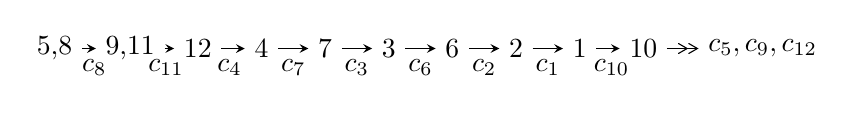
\begin{tikzpicture}[x=23pt, y=7pt]
	% node
	\node (A0) at (-1/8, 0) {5,8};
	\node (A1) at (17/16, 0) {9,11};
	\node (A2) at (17/8, 0) {12};
	\node (A3) at (25/8, 0) {4};
	\node (A4) at (33/8, 0) {7};
	\node (A5) at (41/8, 0) {3};
	\node (A6) at (49/8, 0) {6};
	\node (A7) at (57/8, 0) {2};
	\node (A8) at (65/8, 0) {1};
	\node (A9) at (73/8, 0) {10};
	\node (C1) at (1/2, -1) {$c_{8}$};
	\node (C2) at (13/8, -1) {$c_{11}$};
	\node (C3) at (21/8, -1) {$c_{4}$};
	\node (C4) at (29/8, -1) {$c_{7}$};
	\node (C5) at (37/8, -1) {$c_{3}$};
	\node (C6) at (45/8, -1) {$c_{6}$};
	\node (C7) at (53/8, -1) {$c_{2}$};
	\node (C8) at (61/8, -1) {$c_{1}$};
	\node (C9) at (69/8, -1) {$c_{10}$};
	\node (A10) at (11, 0) {$c_{5},c_{9},c_{12}$};

	% edge
	\draw[->,>=stealth]	
	(A0) edge (A1) (A1) edge (A2) (A2) edge (A3) (A3) edge (A4) (A4) edge (A5) (A5) edge (A6) (A6) edge (A7) (A7) edge (A8) (A8) edge (A9) ;
	\draw[->>,>={angle 60}]	
	(A9) edge (A10);
\end{tikzpicture} \\ 

\end{tabular} \\

\footnotetext{
The image of knot diagram is generated by the software ``\textbf{Draw programme}" developed by Andrew Bartholomew(\url{http://www.layer8.co.uk/maths/draw/index.htm\#Running-draw}), where we modified some parts for our purpose(\url{https://github.com/CATsTAILs/LinksPainter}).
}\phantom \\ \newline 
\centering \textbf{Ideals for irreducible components\footnotemark of $X_{\text{par}}$} 
 
\begin{align*}
I^u_{1}&=\langle 
7.99341\times10^{39} u^{32}-1.73952\times10^{40} u^{31}+\cdots+6.21714\times10^{42} b-7.27832\times10^{42},\\
\phantom{I^u_{1}}&\phantom{= \langle  }-2.58634\times10^{40} u^{32}+4.38348\times10^{40} u^{31}+\cdots+1.24343\times10^{43} a-5.01178\times10^{42},\\
\phantom{I^u_{1}}&\phantom{= \langle  }u^{33}- u^{32}+\cdots+1024 u+512\rangle \\
\\
I^v_{1}&=\langle 
a,\;3 v^5+2 v^4+15 v^3+20 v^2+7 b+12 v-3,\;v^6+v^5+5 v^4+9 v^3+5 v^2+v+1\rangle \\
I^v_{2}&=\langle 
a,\;b^3- b^2+1,\;v-1\rangle \\
\end{align*}
\raggedright * 3 irreducible components of $\dim_{\mathbb{C}}=0$, with total 42 representations.\\
\footnotetext{All coefficients of polynomials are rational numbers. But the coefficients are sometimes approximated in decimal forms when there is not enough margin.}
\newpage
\renewcommand{\arraystretch}{1}
\centering \section*{I. $I^u_{1}= \langle 7.99\times10^{39} u^{32}-1.74\times10^{40} u^{31}+\cdots+6.22\times10^{42} b-7.28\times10^{42},\;-2.59\times10^{40} u^{32}+4.38\times10^{40} u^{31}+\cdots+1.24\times10^{43} a-5.01\times10^{42},\;u^{33}- u^{32}+\cdots+1024 u+512 \rangle$}
\flushleft \textbf{(i) Arc colorings}\\
\begin{tabular}{m{7pt} m{180pt} m{7pt} m{180pt} }
\flushright $a_{5}=$&$\begin{pmatrix}0\\u\end{pmatrix}$ \\
\flushright $a_{8}=$&$\begin{pmatrix}1\\0\end{pmatrix}$ \\
\flushright $a_{9}=$&$\begin{pmatrix}1\\u^2\end{pmatrix}$ \\
\flushright $a_{11}=$&$\begin{pmatrix}0.00208001 u^{32}-0.00352532 u^{31}+\cdots+1.78233 u+0.403062\\-0.00128571 u^{32}+0.00279794 u^{31}+\cdots+1.28986 u+1.17069\end{pmatrix}$ \\
\flushright $a_{12}=$&$\begin{pmatrix}0.000794299 u^{32}-0.000727383 u^{31}+\cdots+3.07219 u+1.57375\\-0.00128571 u^{32}+0.00279794 u^{31}+\cdots+1.28986 u+1.17069\end{pmatrix}$ \\
\flushright $a_{4}=$&$\begin{pmatrix}u\\u^3+u\end{pmatrix}$ \\
\flushright $a_{7}=$&$\begin{pmatrix}-0.00110615 u^{32}+0.00221831 u^{31}+\cdots+0.260315 u+0.865237\\0.00241977 u^{32}-0.00321235 u^{31}+\cdots+4.09026 u+0.856393\end{pmatrix}$ \\
\flushright $a_{3}=$&$\begin{pmatrix}0.00164230 u^{32}-0.00102508 u^{31}+\cdots+3.66559 u+0.647992\\-0.000789549 u^{32}+0.00155917 u^{31}+\cdots+1.76057 u+0.378455\end{pmatrix}$ \\
\flushright $a_{6}=$&$\begin{pmatrix}-0.00110615 u^{32}+0.00221831 u^{31}+\cdots+0.260315 u+0.865237\\0.00119835 u^{32}-0.0000262335 u^{31}+\cdots+4.66276 u+1.42582\end{pmatrix}$ \\
\flushright $a_{2}=$&$\begin{pmatrix}0.00204624 u^{32}-0.0000326376 u^{31}+\cdots+6.09887 u+1.29264\\-0.000664888 u^{32}+0.00290411 u^{31}+\cdots+4.32183 u+1.50071\end{pmatrix}$ \\
\flushright $a_{1}=$&$\begin{pmatrix}0.00230450 u^{32}-0.00224455 u^{31}+\cdots+4.40244 u+0.560582\\0.00119835 u^{32}-0.0000262335 u^{31}+\cdots+4.66276 u+1.42582\end{pmatrix}$ \\
\flushright $a_{10}=$&$\begin{pmatrix}-0.000739170 u^{32}-0.0000503781 u^{31}+\cdots-1.45933 u+1.00366\\-0.00132594 u^{32}+0.00245141 u^{31}+\cdots-0.697988 u+1.25243\end{pmatrix}$\\&\end{tabular}
\flushleft \textbf{(ii) Obstruction class $= -1$}\\~\\
\flushleft \textbf{(iii) Cusp Shapes $= -0.0223829 u^{32}+0.0292513 u^{31}+\cdots-14.9362 u-3.65393$}\\~\\
\newpage\renewcommand{\arraystretch}{1}
\flushleft \textbf{(iv) u-Polynomials at the component}\newline \\
\begin{tabular}{m{50pt}|m{274pt}}
Crossings & \hspace{64pt}u-Polynomials at each crossing \\
\hline $$\begin{aligned}c_{1},c_{6}\end{aligned}$$&$\begin{aligned}
&u^{33}+6 u^{32}+\cdots+2 u+1
\end{aligned}$\\
\hline $$\begin{aligned}c_{2},c_{5}\end{aligned}$$&$\begin{aligned}
&u^{33}+4 u^{32}+\cdots+2 u+1
\end{aligned}$\\
\hline $$\begin{aligned}c_{3}\end{aligned}$$&$\begin{aligned}
&u^{33}-4 u^{32}+\cdots+77426 u+5953
\end{aligned}$\\
\hline $$\begin{aligned}c_{4},c_{8}\end{aligned}$$&$\begin{aligned}
&u^{33}- u^{32}+\cdots+1024 u+512
\end{aligned}$\\
\hline $$\begin{aligned}c_{7},c_{11}\end{aligned}$$&$\begin{aligned}
&u^{33}-4 u^{32}+\cdots+2 u+1
\end{aligned}$\\
\hline $$\begin{aligned}c_{9}\end{aligned}$$&$\begin{aligned}
&u^{33}+4 u^{32}+\cdots-18 u+1
\end{aligned}$\\
\hline $$\begin{aligned}c_{10},c_{12}\end{aligned}$$&$\begin{aligned}
&u^{33}-14 u^{32}+\cdots+50 u-1
\end{aligned}$\\
\hline
\end{tabular}\\~\\
\newpage\renewcommand{\arraystretch}{1}
\flushleft \textbf{(v) Riley Polynomials at the component}\newline \\
\begin{tabular}{m{50pt}|m{274pt}}
Crossings & \hspace{64pt}Riley Polynomials at each crossing \\
\hline $$\begin{aligned}c_{1},c_{6}\end{aligned}$$&$\begin{aligned}
&y^{33}+46 y^{32}+\cdots+66 y-1
\end{aligned}$\\
\hline $$\begin{aligned}c_{2},c_{5}\end{aligned}$$&$\begin{aligned}
&y^{33}-6 y^{32}+\cdots+2 y-1
\end{aligned}$\\
\hline $$\begin{aligned}c_{3}\end{aligned}$$&$\begin{aligned}
&y^{33}+130 y^{32}+\cdots+1530880802 y-35438209
\end{aligned}$\\
\hline $$\begin{aligned}c_{4},c_{8}\end{aligned}$$&$\begin{aligned}
&y^{33}+49 y^{32}+\cdots-917504 y-262144
\end{aligned}$\\
\hline $$\begin{aligned}c_{7},c_{11}\end{aligned}$$&$\begin{aligned}
&y^{33}-14 y^{32}+\cdots+50 y-1
\end{aligned}$\\
\hline $$\begin{aligned}c_{9}\end{aligned}$$&$\begin{aligned}
&y^{33}-70 y^{32}+\cdots+290 y-1
\end{aligned}$\\
\hline $$\begin{aligned}c_{10},c_{12}\end{aligned}$$&$\begin{aligned}
&y^{33}+14 y^{32}+\cdots+1938 y-1
\end{aligned}$\\
\hline
\end{tabular}\\~\\
\newpage\flushleft \textbf{(vi) Complex Volumes and Cusp Shapes}
$$\begin{array}{c|c|c}  
\text{Solutions to }I^u_{1}& \I (\text{vol} + \sqrt{-1}CS) & \text{Cusp shape}\\
 \hline 
\begin{aligned}
u &= -0.259194 + 0.938083 I \\
a &= \phantom{-}1.296390 - 0.418631 I \\
b &= -0.842802 + 0.497518 I\end{aligned}
 & -1.68399 - 2.04132 I & -4.24848 + 3.69259 I \\ \hline\begin{aligned}
u &= -0.259194 - 0.938083 I \\
a &= \phantom{-}1.296390 + 0.418631 I \\
b &= -0.842802 - 0.497518 I\end{aligned}
 & -1.68399 + 2.04132 I & -4.24848 - 3.69259 I \\ \hline\begin{aligned}
u &= -0.299553 + 0.982584 I \\
a &= \phantom{-}0.491758 - 0.071067 I \\
b &= -0.276643 - 0.578301 I\end{aligned}
 & \phantom{-}1.95211 + 1.67358 I & -0.85105 - 3.68739 I \\ \hline\begin{aligned}
u &= -0.299553 - 0.982584 I \\
a &= \phantom{-}0.491758 + 0.071067 I \\
b &= -0.276643 + 0.578301 I\end{aligned}
 & \phantom{-}1.95211 - 1.67358 I & -0.85105 + 3.68739 I \\ \hline\begin{aligned}
u &= -0.819751 + 0.642390 I \\
a &= -1.19497 + 1.76483 I \\
b &= \phantom{-}0.940469 + 0.288411 I\end{aligned}
 & \phantom{-}4.57287 - 1.92834 I & \phantom{-}2.42456 - 1.90294 I \\ \hline\begin{aligned}
u &= -0.819751 - 0.642390 I \\
a &= -1.19497 - 1.76483 I \\
b &= \phantom{-}0.940469 - 0.288411 I\end{aligned}
 & \phantom{-}4.57287 + 1.92834 I & \phantom{-}2.42456 + 1.90294 I \\ \hline\begin{aligned}
u &= \phantom{-}0.906320 + 0.161254 I \\
a &= -0.342325 + 1.004680 I \\
b &= \phantom{-}0.936395 + 0.663389 I\end{aligned}
 & -1.64047 + 4.33466 I & -2.39244 - 5.76520 I \\ \hline\begin{aligned}
u &= \phantom{-}0.906320 - 0.161254 I \\
a &= -0.342325 - 1.004680 I \\
b &= \phantom{-}0.936395 - 0.663389 I\end{aligned}
 & -1.64047 - 4.33466 I & -2.39244 + 5.76520 I \\ \hline\begin{aligned}
u &= -0.138715 + 1.076100 I \\
a &= \phantom{-}0.343138 - 0.314662 I \\
b &= -0.540873 + 0.646097 I\end{aligned}
 & \phantom{-}0.99056 + 3.01055 I & -2.29192 - 3.36152 I \\ \hline\begin{aligned}
u &= -0.138715 - 1.076100 I \\
a &= \phantom{-}0.343138 + 0.314662 I \\
b &= -0.540873 - 0.646097 I\end{aligned}
 & \phantom{-}0.99056 - 3.01055 I & -2.29192 + 3.36152 I\\
 \hline 
 \end{array}$$\newpage$$\begin{array}{c|c|c}  
\text{Solutions to }I^u_{1}& \I (\text{vol} + \sqrt{-1}CS) & \text{Cusp shape}\\
 \hline 
\begin{aligned}
u &= -0.820423 + 0.241734 I \\
a &= -0.127283 + 1.097200 I \\
b &= \phantom{-}0.790989 + 0.648302 I\end{aligned}
 & -2.09854 + 0.79204 I & -4.42932 + 0.29217 I \\ \hline\begin{aligned}
u &= -0.820423 - 0.241734 I \\
a &= -0.127283 - 1.097200 I \\
b &= \phantom{-}0.790989 - 0.648302 I\end{aligned}
 & -2.09854 - 0.79204 I & -4.42932 - 0.29217 I \\ \hline\begin{aligned}
u &= \phantom{-}0.588887 + 0.452734 I \\
a &= \phantom{-}1.005150 + 0.039063 I \\
b &= -0.876518 - 0.152706 I\end{aligned}
 & \phantom{-}1.49526 + 0.33133 I & \phantom{-}5.50598 - 0.36289 I \\ \hline\begin{aligned}
u &= \phantom{-}0.588887 - 0.452734 I \\
a &= \phantom{-}1.005150 - 0.039063 I \\
b &= -0.876518 + 0.152706 I\end{aligned}
 & \phantom{-}1.49526 - 0.33133 I & \phantom{-}5.50598 + 0.36289 I \\ \hline\begin{aligned}
u &= \phantom{-}1.103600 + 0.681610 I \\
a &= -1.01014 - 1.30375 I \\
b &= \phantom{-}1.017310 - 0.360748 I\end{aligned}
 & \phantom{-}5.11059 - 4.16082 I & \phantom{-}2.72191 + 5.85960 I \\ \hline\begin{aligned}
u &= \phantom{-}1.103600 - 0.681610 I \\
a &= -1.01014 + 1.30375 I \\
b &= \phantom{-}1.017310 + 0.360748 I\end{aligned}
 & \phantom{-}5.11059 + 4.16082 I & \phantom{-}2.72191 - 5.85960 I \\ \hline\begin{aligned}
u &= -0.020434 + 1.399020 I \\
a &= \phantom{-}1.58993 + 0.37908 I \\
b &= -1.035370 + 0.580512 I\end{aligned}
 & \phantom{-}2.46612 - 7.83728 I & \phantom{-}0.08663 + 7.57867 I \\ \hline\begin{aligned}
u &= -0.020434 - 1.399020 I \\
a &= \phantom{-}1.58993 - 0.37908 I \\
b &= -1.035370 - 0.580512 I\end{aligned}
 & \phantom{-}2.46612 + 7.83728 I & \phantom{-}0.08663 - 7.57867 I \\ \hline\begin{aligned}
u &= -0.023074 + 0.498558 I \\
a &= -0.216617 + 0.905947 I \\
b &= \phantom{-}0.878924 + 0.769382 I\end{aligned}
 & -3.74171 + 2.90167 I & \phantom{-}6.31914 - 4.62545 I \\ \hline\begin{aligned}
u &= -0.023074 - 0.498558 I \\
a &= -0.216617 - 0.905947 I \\
b &= \phantom{-}0.878924 - 0.769382 I\end{aligned}
 & -3.74171 - 2.90167 I & \phantom{-}6.31914 + 4.62545 I\\
 \hline 
 \end{array}$$\newpage$$\begin{array}{c|c|c}  
\text{Solutions to }I^u_{1}& \I (\text{vol} + \sqrt{-1}CS) & \text{Cusp shape}\\
 \hline 
\begin{aligned}
u &= \phantom{-}0.38369 + 1.47441 I \\
a &= \phantom{-}1.321050 - 0.219840 I \\
b &= -1.068020 - 0.492605 I\end{aligned}
 & \phantom{-}4.14146 + 2.52091 I & \phantom{-}3.12902 - 2.10165 I \\ \hline\begin{aligned}
u &= \phantom{-}0.38369 - 1.47441 I \\
a &= \phantom{-}1.321050 + 0.219840 I \\
b &= -1.068020 + 0.492605 I\end{aligned}
 & \phantom{-}4.14146 - 2.52091 I & \phantom{-}3.12902 + 2.10165 I \\ \hline\begin{aligned}
u &= -0.379202\phantom{ +0.000000I} \\
a &= \phantom{-}1.20462\phantom{ +0.000000I} \\
b &= \phantom{-}0.150542\phantom{ +0.000000I}\end{aligned}
 & -0.908337\phantom{ +0.000000I} & -11.6530\phantom{ +0.000000I} \\ \hline\begin{aligned}
u &= -0.43213 + 1.91828 I \\
a &= -0.064840 + 0.127886 I \\
b &= -0.511933 + 0.957121 I\end{aligned}
 & \phantom{-}11.27410 + 6.04297 I & \phantom{-0.000000 } 0 \\ \hline\begin{aligned}
u &= -0.43213 - 1.91828 I \\
a &= -0.064840 - 0.127886 I \\
b &= -0.511933 - 0.957121 I\end{aligned}
 & \phantom{-}11.27410 - 6.04297 I & \phantom{-0.000000 } 0 \\ \hline\begin{aligned}
u &= \phantom{-}0.27574 + 1.97448 I \\
a &= -0.016267 - 0.141101 I \\
b &= -0.473285 - 0.959466 I\end{aligned}
 & \phantom{-}11.52690 + 0.81316 I & \phantom{-0.000000 } 0 \\ \hline\begin{aligned}
u &= \phantom{-}0.27574 - 1.97448 I \\
a &= -0.016267 + 0.141101 I \\
b &= -0.473285 + 0.959466 I\end{aligned}
 & \phantom{-}11.52690 - 0.81316 I & \phantom{-0.000000 } 0 \\ \hline\begin{aligned}
u &= \phantom{-}0.66557 + 1.97108 I \\
a &= \phantom{-}1.118020 + 0.848015 I \\
b &= -1.143380 + 0.700941 I\end{aligned}
 & \phantom{-}13.2296 - 12.1129 I & \phantom{-0.000000 } 0 \\ \hline\begin{aligned}
u &= \phantom{-}0.66557 - 1.97108 I \\
a &= \phantom{-}1.118020 - 0.848015 I \\
b &= -1.143380 - 0.700941 I\end{aligned}
 & \phantom{-}13.2296 + 12.1129 I & \phantom{-0.000000 } 0 \\ \hline\begin{aligned}
u &= -0.53201 + 2.07441 I \\
a &= \phantom{-}1.114790 - 0.764503 I \\
b &= -1.158540 - 0.681377 I\end{aligned}
 & \phantom{-}13.6520 + 5.1893 I & \phantom{-0.000000 } 0\\
 \hline 
 \end{array}$$\newpage$$\begin{array}{c|c|c}  
\text{Solutions to }I^u_{1}& \I (\text{vol} + \sqrt{-1}CS) & \text{Cusp shape}\\
 \hline 
\begin{aligned}
u &= -0.53201 - 2.07441 I \\
a &= \phantom{-}1.114790 + 0.764503 I \\
b &= -1.158540 + 0.681377 I\end{aligned}
 & \phantom{-}13.6520 - 5.1893 I & \phantom{-0.000000 } 0 \\ \hline\begin{aligned}
u &= \phantom{-}0.11108 + 2.30479 I \\
a &= -1.410100 - 0.047794 I \\
b &= \phantom{-}1.288010 - 0.018877 I\end{aligned}
 & \phantom{-}18.1642 - 3.5486 I & \phantom{-0.000000 } 0 \\ \hline\begin{aligned}
u &= \phantom{-}0.11108 - 2.30479 I \\
a &= -1.410100 + 0.047794 I \\
b &= \phantom{-}1.288010 + 0.018877 I\end{aligned}
 & \phantom{-}18.1642 + 3.5486 I & \phantom{-0.000000 } 0\\
 \hline 
 \end{array}$$\newpage\newpage\renewcommand{\arraystretch}{1}
\centering \section*{II. $I^v_{1}= \langle a,\;3 v^5+2 v^4+15 v^3+20 v^2+7 b+12 v-3,\;v^6+v^5+5 v^4+9 v^3+5 v^2+v+1 \rangle$}
\flushleft \textbf{(i) Arc colorings}\\
\begin{tabular}{m{7pt} m{180pt} m{7pt} m{180pt} }
\flushright $a_{5}=$&$\begin{pmatrix}v\\0\end{pmatrix}$ \\
\flushright $a_{8}=$&$\begin{pmatrix}1\\0\end{pmatrix}$ \\
\flushright $a_{9}=$&$\begin{pmatrix}1\\0\end{pmatrix}$ \\
\flushright $a_{11}=$&$\begin{pmatrix}0\\-\frac{3}{7} v^5-\frac{2}{7} v^4+\cdots-\frac{12}{7} v+\frac{3}{7}\end{pmatrix}$ \\
\flushright $a_{12}=$&$\begin{pmatrix}-\frac{3}{7} v^5-\frac{2}{7} v^4+\cdots-\frac{12}{7} v+\frac{3}{7}\\-\frac{3}{7} v^5-\frac{2}{7} v^4+\cdots-\frac{12}{7} v+\frac{3}{7}\end{pmatrix}$ \\
\flushright $a_{4}=$&$\begin{pmatrix}v\\0\end{pmatrix}$ \\
\flushright $a_{7}=$&$\begin{pmatrix}1\\-\frac{5}{7} v^5-\frac{3}{7} v^4+\cdots-3 v-\frac{4}{7}\end{pmatrix}$ \\
\flushright $a_{3}=$&$\begin{pmatrix}-\frac{2}{7} v^5+\frac{1}{7} v^4+\cdots+\frac{6}{7} v-\frac{5}{7}\\-\frac{1}{7} v^5+\frac{1}{7} v^4+\cdots+\frac{12}{7} v-\frac{2}{7}\end{pmatrix}$ \\
\flushright $a_{6}=$&$\begin{pmatrix}-\frac{3}{7} v^5-2 v^3+\cdots+\frac{3}{7} v+\frac{5}{7}\\-\frac{5}{7} v^5-\frac{3}{7} v^4+\cdots-3 v-\frac{4}{7}\end{pmatrix}$ \\
\flushright $a_{2}=$&$\begin{pmatrix}-\frac{1}{7} v^5+\frac{2}{7} v^4+\cdots+\frac{2}{7} v-\frac{8}{7}\\\frac{1}{7} v^5+\frac{5}{7} v^4+\cdots+\frac{26}{7} v+\frac{1}{7}\end{pmatrix}$ \\
\flushright $a_{1}=$&$\begin{pmatrix}-1\\\frac{5}{7} v^5+\frac{3}{7} v^4+\cdots+3 v+\frac{4}{7}\end{pmatrix}$ \\
\flushright $a_{10}=$&$\begin{pmatrix}\frac{5}{7} v^5+\frac{3}{7} v^4+\cdots+3 v+\frac{11}{7}\\\frac{2}{7} v^5+\frac{1}{7} v^4+\cdots+\frac{9}{7} v+2\end{pmatrix}$\\&\end{tabular}
\flushleft \textbf{(ii) Obstruction class $= 1$}\\~\\
\flushleft \textbf{(iii) Cusp Shapes $= 5 v^5+\frac{12}{7} v^4+\frac{160}{7} v^3+\frac{199}{7} v^2+\frac{20}{7} v-\frac{58}{7}$}\\~\\
\newpage\renewcommand{\arraystretch}{1}
\flushleft \textbf{(iv) u-Polynomials at the component}\newline \\
\begin{tabular}{m{50pt}|m{274pt}}
Crossings & \hspace{64pt}u-Polynomials at each crossing \\
\hline $$\begin{aligned}c_{1},c_{3},c_{9}\\c_{12}\end{aligned}$$&$\begin{aligned}
&(u^3- u^2+2 u-1)^2
\end{aligned}$\\
\hline $$\begin{aligned}c_{2},c_{11}\end{aligned}$$&$\begin{aligned}
&(u^3+u^2-1)^2
\end{aligned}$\\
\hline $$\begin{aligned}c_{4},c_{8}\end{aligned}$$&$\begin{aligned}
&u^6
\end{aligned}$\\
\hline $$\begin{aligned}c_{5},c_{7}\end{aligned}$$&$\begin{aligned}
&(u^3- u^2+1)^2
\end{aligned}$\\
\hline $$\begin{aligned}c_{6},c_{10}\end{aligned}$$&$\begin{aligned}
&(u^3+u^2+2 u+1)^2
\end{aligned}$\\
\hline
\end{tabular}\\~\\
\newpage\renewcommand{\arraystretch}{1}
\flushleft \textbf{(v) Riley Polynomials at the component}\newline \\
\begin{tabular}{m{50pt}|m{274pt}}
Crossings & \hspace{64pt}Riley Polynomials at each crossing \\
\hline $$\begin{aligned}c_{1},c_{3},c_{6}\\c_{9},c_{10},c_{12}\end{aligned}$$&$\begin{aligned}
&(y^3+3 y^2+2 y-1)^2
\end{aligned}$\\
\hline $$\begin{aligned}c_{2},c_{5},c_{7}\\c_{11}\end{aligned}$$&$\begin{aligned}
&(y^3- y^2+2 y-1)^2
\end{aligned}$\\
\hline $$\begin{aligned}c_{4},c_{8}\end{aligned}$$&$\begin{aligned}
&y^6
\end{aligned}$\\
\hline
\end{tabular}\\~\\
\newpage\flushleft \textbf{(vi) Complex Volumes and Cusp Shapes}
$$\begin{array}{c|c|c}  
\text{Solutions to }I^v_{1}& \I (\text{vol} + \sqrt{-1}CS) & \text{Cusp shape}\\
 \hline 
\begin{aligned}
v &= -0.947279 + 0.320410 I \\
a &= \phantom{-0.000000 } 0 \\
b &= \phantom{-}0.877439 - 0.744862 I\end{aligned}
 & \phantom{-0.000000 } -5.65624 I & -0.41065 + 5.95889 I \\ \hline\begin{aligned}
v &= -0.947279 - 0.320410 I \\
a &= \phantom{-0.000000 } 0 \\
b &= \phantom{-}0.877439 + 0.744862 I\end{aligned}
 & \phantom{-0.000000 -}5.65624 I & -0.41065 - 5.95889 I \\ \hline\begin{aligned}
v &= \phantom{-}0.069840 + 0.424452 I \\
a &= \phantom{-0.000000 } 0 \\
b &= \phantom{-}0.877439 - 0.744862 I\end{aligned}
 & -4.13758 - 2.82812 I & -13.82394 + 1.30714 I \\ \hline\begin{aligned}
v &= \phantom{-}0.069840 - 0.424452 I \\
a &= \phantom{-0.000000 } 0 \\
b &= \phantom{-}0.877439 + 0.744862 I\end{aligned}
 & -4.13758 + 2.82812 I & -13.82394 - 1.30714 I \\ \hline\begin{aligned}
v &= \phantom{-}0.37744 + 2.29387 I \\
a &= \phantom{-0.000000 } 0 \\
b &= -0.754878\phantom{ +0.000000I}\end{aligned}
 & \phantom{-}4.13758 - 2.82812 I & -0.76541 + 4.65175 I \\ \hline\begin{aligned}
v &= \phantom{-}0.37744 - 2.29387 I \\
a &= \phantom{-0.000000 } 0 \\
b &= -0.754878\phantom{ +0.000000I}\end{aligned}
 & \phantom{-}4.13758 + 2.82812 I & -0.76541 - 4.65175 I\\
 \hline 
 \end{array}$$\newpage\newpage\renewcommand{\arraystretch}{1}
\centering \section*{III. $I^v_{2}= \langle a,\;b^3- b^2+1,\;v-1 \rangle$}
\flushleft \textbf{(i) Arc colorings}\\
\begin{tabular}{m{7pt} m{180pt} m{7pt} m{180pt} }
\flushright $a_{5}=$&$\begin{pmatrix}1\\0\end{pmatrix}$ \\
\flushright $a_{8}=$&$\begin{pmatrix}1\\0\end{pmatrix}$ \\
\flushright $a_{9}=$&$\begin{pmatrix}1\\0\end{pmatrix}$ \\
\flushright $a_{11}=$&$\begin{pmatrix}0\\b\end{pmatrix}$ \\
\flushright $a_{12}=$&$\begin{pmatrix}b\\b\end{pmatrix}$ \\
\flushright $a_{4}=$&$\begin{pmatrix}1\\0\end{pmatrix}$ \\
\flushright $a_{7}=$&$\begin{pmatrix}1\\b^2\end{pmatrix}$ \\
\flushright $a_{3}=$&$\begin{pmatrix}- b^2+1\\- b^2+b+1\end{pmatrix}$ \\
\flushright $a_{6}=$&$\begin{pmatrix}b^2+1\\b^2\end{pmatrix}$ \\
\flushright $a_{2}=$&$\begin{pmatrix}b\\b\end{pmatrix}$ \\
\flushright $a_{1}=$&$\begin{pmatrix}-1\\- b^2\end{pmatrix}$ \\
\flushright $a_{10}=$&$\begin{pmatrix}- b^2+1\\- b^2+b+1\end{pmatrix}$\\&\end{tabular}
\flushleft \textbf{(ii) Obstruction class $= 1$}\\~\\
\flushleft \textbf{(iii) Cusp Shapes $= 0$}\\~\\
\newpage\renewcommand{\arraystretch}{1}
\flushleft \textbf{(iv) u-Polynomials at the component}\newline \\
\begin{tabular}{m{50pt}|m{274pt}}
Crossings & \hspace{64pt}u-Polynomials at each crossing \\
\hline $$\begin{aligned}c_{1},c_{3},c_{9}\\c_{12}\end{aligned}$$&$\begin{aligned}
&u^3- u^2+2 u-1
\end{aligned}$\\
\hline $$\begin{aligned}c_{2},c_{11}\end{aligned}$$&$\begin{aligned}
&u^3+u^2-1
\end{aligned}$\\
\hline $$\begin{aligned}c_{4},c_{8}\end{aligned}$$&$\begin{aligned}
&u^3
\end{aligned}$\\
\hline $$\begin{aligned}c_{5},c_{7}\end{aligned}$$&$\begin{aligned}
&u^3- u^2+1
\end{aligned}$\\
\hline $$\begin{aligned}c_{6},c_{10}\end{aligned}$$&$\begin{aligned}
&u^3+u^2+2 u+1
\end{aligned}$\\
\hline
\end{tabular}\\~\\
\newpage\renewcommand{\arraystretch}{1}
\flushleft \textbf{(v) Riley Polynomials at the component}\newline \\
\begin{tabular}{m{50pt}|m{274pt}}
Crossings & \hspace{64pt}Riley Polynomials at each crossing \\
\hline $$\begin{aligned}c_{1},c_{3},c_{6}\\c_{9},c_{10},c_{12}\end{aligned}$$&$\begin{aligned}
&y^3+3 y^2+2 y-1
\end{aligned}$\\
\hline $$\begin{aligned}c_{2},c_{5},c_{7}\\c_{11}\end{aligned}$$&$\begin{aligned}
&y^3- y^2+2 y-1
\end{aligned}$\\
\hline $$\begin{aligned}c_{4},c_{8}\end{aligned}$$&$\begin{aligned}
&y^3
\end{aligned}$\\
\hline
\end{tabular}\\~\\
\newpage\flushleft \textbf{(vi) Complex Volumes and Cusp Shapes}
$$\begin{array}{c|c|c}  
\text{Solutions to }I^v_{2}& \I (\text{vol} + \sqrt{-1}CS) & \text{Cusp shape}\\
 \hline 
\begin{aligned}
v &= \phantom{-}1.00000\phantom{ +0.000000I} \\
a &= \phantom{-0.000000 } 0 \\
b &= \phantom{-}0.877439 + 0.744862 I\end{aligned}
 & \phantom{-0.000000 } 0 & \phantom{-0.000000 } 0 \\ \hline\begin{aligned}
v &= \phantom{-}1.00000\phantom{ +0.000000I} \\
a &= \phantom{-0.000000 } 0 \\
b &= \phantom{-}0.877439 - 0.744862 I\end{aligned}
 & \phantom{-0.000000 } 0 & \phantom{-0.000000 } 0 \\ \hline\begin{aligned}
v &= \phantom{-}1.00000\phantom{ +0.000000I} \\
a &= \phantom{-0.000000 } 0 \\
b &= -0.754878\phantom{ +0.000000I}\end{aligned}
 & \phantom{-0.000000 } 0 & \phantom{-0.000000 } 0\\
 \hline 
 \end{array}$$\newpage
\newpage\renewcommand{\arraystretch}{1}
\centering \section*{ IV. u-Polynomials}
\begin{tabular}{m{50pt}|m{274pt}}
Crossings & \hspace{64pt}u-Polynomials at each crossing \\
\hline $$\begin{aligned}c_{1}\end{aligned}$$&$\begin{aligned}
&((u^3- u^2+2 u-1)^3)(u^{33}+6 u^{32}+\cdots+2 u+1)
\end{aligned}$\\
\hline $$\begin{aligned}c_{2}\end{aligned}$$&$\begin{aligned}
&((u^3+u^2-1)^3)(u^{33}+4 u^{32}+\cdots+2 u+1)
\end{aligned}$\\
\hline $$\begin{aligned}c_{3}\end{aligned}$$&$\begin{aligned}
&((u^3- u^2+2 u-1)^3)(u^{33}-4 u^{32}+\cdots+77426 u+5953)
\end{aligned}$\\
\hline $$\begin{aligned}c_{4},c_{8}\end{aligned}$$&$\begin{aligned}
&u^9(u^{33}- u^{32}+\cdots+1024 u+512)
\end{aligned}$\\
\hline $$\begin{aligned}c_{5}\end{aligned}$$&$\begin{aligned}
&((u^3- u^2+1)^3)(u^{33}+4 u^{32}+\cdots+2 u+1)
\end{aligned}$\\
\hline $$\begin{aligned}c_{6}\end{aligned}$$&$\begin{aligned}
&((u^3+u^2+2 u+1)^3)(u^{33}+6 u^{32}+\cdots+2 u+1)
\end{aligned}$\\
\hline $$\begin{aligned}c_{7}\end{aligned}$$&$\begin{aligned}
&((u^3- u^2+1)^3)(u^{33}-4 u^{32}+\cdots+2 u+1)
\end{aligned}$\\
\hline $$\begin{aligned}c_{9}\end{aligned}$$&$\begin{aligned}
&((u^3- u^2+2 u-1)^3)(u^{33}+4 u^{32}+\cdots-18 u+1)
\end{aligned}$\\
\hline $$\begin{aligned}c_{10}\end{aligned}$$&$\begin{aligned}
&((u^3+u^2+2 u+1)^3)(u^{33}-14 u^{32}+\cdots+50 u-1)
\end{aligned}$\\
\hline $$\begin{aligned}c_{11}\end{aligned}$$&$\begin{aligned}
&((u^3+u^2-1)^3)(u^{33}-4 u^{32}+\cdots+2 u+1)
\end{aligned}$\\
\hline $$\begin{aligned}c_{12}\end{aligned}$$&$\begin{aligned}
&((u^3- u^2+2 u-1)^3)(u^{33}-14 u^{32}+\cdots+50 u-1)
\end{aligned}$\\
\hline
\end{tabular}\newpage\renewcommand{\arraystretch}{1}
\centering \section*{ V. Riley Polynomials}
\begin{tabular}{m{50pt}|m{274pt}}
Crossings & \hspace{64pt}Riley Polynomials at each crossing \\
\hline $$\begin{aligned}c_{1},c_{6}\end{aligned}$$&$\begin{aligned}
&((y^3+3 y^2+2 y-1)^3)(y^{33}+46 y^{32}+\cdots+66 y-1)
\end{aligned}$\\
\hline $$\begin{aligned}c_{2},c_{5}\end{aligned}$$&$\begin{aligned}
&((y^3- y^2+2 y-1)^3)(y^{33}-6 y^{32}+\cdots+2 y-1)
\end{aligned}$\\
\hline $$\begin{aligned}c_{3}\end{aligned}$$&$\begin{aligned}
&(y^3+3 y^2+2 y-1)^3\\
&\cdot(y^{33}+130 y^{32}+\cdots+1530880802 y-35438209)
\end{aligned}$\\
\hline $$\begin{aligned}c_{4},c_{8}\end{aligned}$$&$\begin{aligned}
&y^9(y^{33}+49 y^{32}+\cdots-917504 y-262144)
\end{aligned}$\\
\hline $$\begin{aligned}c_{7},c_{11}\end{aligned}$$&$\begin{aligned}
&((y^3- y^2+2 y-1)^3)(y^{33}-14 y^{32}+\cdots+50 y-1)
\end{aligned}$\\
\hline $$\begin{aligned}c_{9}\end{aligned}$$&$\begin{aligned}
&((y^3+3 y^2+2 y-1)^3)(y^{33}-70 y^{32}+\cdots+290 y-1)
\end{aligned}$\\
\hline $$\begin{aligned}c_{10},c_{12}\end{aligned}$$&$\begin{aligned}
&((y^3+3 y^2+2 y-1)^3)(y^{33}+14 y^{32}+\cdots+1938 y-1)
\end{aligned}$\\
\hline
\end{tabular}
\vskip 2pc
\end{document}